\documentclass{article}
\usepackage{graphicx} % Required for inserting images
\usepackage{subcaption}
\usepackage[authoryear]{natbib}
\usepackage{amsmath}
\usepackage{booktabs}

\title{Multi-modal MRI for Identifying Lymphovascular Invasion in Endometrial Cancer}
\author{Puzhu Wang}
\date{March 2026}

\begin{document}

\maketitle

\subsection{Literature Review}
\label{sec:harmonization-integration}

Radiomics provides a quantitative characterization of tumor phenotype through
high-dimensional features describing intensity, shape, texture, and spatial
heterogeneity. In multi-sequence magnetic resonance imaging (MRI), the imaging
sequences offer related but nonredundant descriptions of the same tumor. T1-
and T2-weighted images characterize different aspects of anatomy and tissue
composition, whereas apparent diffusion coefficient (ADC) images quantify
water diffusion and may provide information related to tumor cellularity.
Joint analysis of these complementary measurements can therefore provide a
more complete description of tumor heterogeneity than separate analyses of
the individual sequences. More broadly, the multi-view and multi-omics
literature has shown that integrating complementary data sources can reveal
coordinated sources of variation, facilitate patient stratification, and
support biomarker discovery \citep{subramanian2020multiomics,
vahabi2022unsupervised}.

A central challenge in multicenter radiomic analysis is that extracted
features reflect technical as well as biological variation. Scanner
manufacturer, magnetic-field strength, acquisition and reconstruction
parameters, voxel size, segmentation procedures, and intensity preprocessing
can affect feature distributions and reproducibility
\citep{mali2021radiomics}. Consequently, directly pooling radiomic features
across centers can introduce systematic location and scale differences. When
these technical effects are large, unsupervised dimension reduction and
clustering may primarily distinguish imaging centers rather than clinically
meaningful tumor phenotypes. Multisite MRI studies have similarly demonstrated
that scanner effects can dominate major directions of variation and reduce the
reproducibility of downstream analyses \citep{fortin2018cortical}.

ComBat was originally introduced as an empirical Bayes method for correcting
batch effects in high-dimensional genomic data \citep{johnson2007combat}. For
each feature, it estimates batch-specific additive and multiplicative effects
while borrowing information across features to stabilize estimation. ComBat
was subsequently adapted to medical imaging and radiomics.
For example, \citet{orlhac2018postreconstruction} reported that ComBat reduced
center-associated differences in PET radiomic features while retaining
patient-specific variation, and \citet{fortin2018cortical} demonstrated the
removal of scanner-associated location and scale effects in multicenter MRI.
Subsequent studies further showed that ComBat and its extensions can improve
radiomic-feature comparability and support the development of more
reproducible multicenter models
\citep{daano2020combat,masson2021harmonization}.

Harmonization alone, however, does not integrate information across MRI
sequences. After center correction, the T1, T2, and ADC measurements remain
separate high-dimensional feature matrices. Direct feature concatenation is a
simple integration strategy, but it can allow a modality with more features or
greater residual variance to dominate the analysis. It also does not explicitly
distinguish variation shared across modalities from variation specific to one
modality. These limitations motivate structured latent-variable methods for
multimodal integration.

Integrative clustering methods identify sample subgroups by jointly analyzing
multiple high-dimensional modalities. A recent review by
\citet{li2026integrative} organizes these methods into approaches based on
shared latent representations, probabilistic dependence among
modality-specific clusterings, and fusion of sample-similarity structures. One
widely used strategy is to first estimate a low-dimensional representation
shared across modalities and then cluster the estimated scores. The iCluster
framework introduced a joint latent-variable model linking multiple genomic
data types through common sample-level factors \citep{shen2009icluster}.
Extensions incorporated heterogeneous outcome distributions and sparse feature
selection \citep{mo2013pattern}, as well as fully Bayesian inference
\citep{mo2018bayesian}. Similarly, Joint and Individual Variation Explained
(JIVE) decomposes linked datasets into joint structure, modality-specific
structure, and residual noise \citep{lock2013jive}; clustering the joint and
individual components can reveal shared and modality-specific subgroups,
respectively \citep{hellton2016integrative}.

A second family of methods estimates related but potentially distinct
clusterings for the individual modalities. Bayesian correlated clustering
models dependence between modality-specific cluster memberships
\citep{kirk2012bayesian}, whereas Bayesian consensus clustering shrinks the
modality-specific partitions toward an overall sample partition
\citep{lock2013consensus}. Clusternomics permits more heterogeneous
cross-modality structure by modeling both local and global clusters with a
hierarchical Dirichlet mixture model \citep{gabasova2017clusternomics}. A third
family integrates sample similarities rather than the original features.
Similarity Network Fusion constructs a sample-similarity network for each
modality and iteratively combines the networks before clustering
\citep{wang2014snf}. Such similarity-based approaches can accommodate
modality-specific distance measures and nonlinear neighborhood structure.

Among shared-latent-representation approaches, Multi-Omics Factor Analysis
(MOFA) provides a general probabilistic multi-view factor model. Although it
was originally developed for multi-omics data, its formulation is applicable
to other aligned, high-dimensional modalities, including radiomic feature
sets. For modality $m$, the model can be summarized as
\begin{equation}
    \mathbf{X}^{(m)} = \mathbf{Z}\mathbf{W}^{(m)\mathsf{T}}
    + \mathbf{E}^{(m)},
\end{equation}
where $\mathbf{Z}$ contains patient-level factor scores,
$\mathbf{W}^{(m)}$ contains modality-specific feature weights, and
$\mathbf{E}^{(m)}$ contains residual variation. Sparsity-inducing and automatic
relevance determination priors allow a factor to explain variation shared by
several modalities or variation concentrated in a single modality
\citep{argelaguet2018mofa}. MOFA+ extends this framework with more scalable
variational inference and group-wise regularization for jointly modeling
multiple groups or experimental conditions \citep{argelaguet2020mofaplus}.
It can also accommodate partially overlapping sample sets and missing
observations; nevertheless, reliable cross-modal integration requires aligned
sample identities or sufficient overlap to connect the modalities.

Taken together, this literature distinguishes two complementary statistical
objectives. Harmonization methods such as ComBat target known technical
variation across acquisition environments, whereas multi-view factor models
such as MOFA characterize covariance shared across or specific to different
modalities. Their sequential use may reduce the influence of technical effects
on the learned representation while retaining the interpretability of latent
factors and modality-specific feature weights. However, neither harmonization
nor latent-factor estimation guarantees biological validity. Center may be
confounded with patient composition, harmonization may attenuate meaningful
variation, and factors explaining substantial variance need not be clinically
relevant. These limitations motivate explicit evaluation of technical-effect
removal and the stability of the resulting factors and clusters.


\section{Methods}
\subsection{Methods: Harmonization and Multimodal Integration}
\label{sec:multimodal-methods}

\subsubsection{Data organization and preprocessing}

The dataset used in this study was collected by the Affiliated Hospital of Nanjing University of Chinese Medicine from two clinical centers over a specified period, with appropriate patient consent and authorization for public use. The original MRI signals were preprocessed following a multiparametric MRI-based radiomics pipeline \citep{cao2024multiparameter}, implemented by one of the original contributors, Jingya Chen, who is in the Department of Radiology at the Affiliated Hospital of Nanjing University of Chinese Medicine.

Radiomic features were extracted from the T1-, T2-, and ADC-weighted MRI sequences and organized as three patient-by-feature matrices. Patient identifiers were aligned across modalities so that corresponding rows referred
to the same patient. Features with unusable or missing measurements were handled before model fitting, and the same feature definitions and ordering were retained across imaging centers. All preprocessing was performed separately by modality to preserve the multi-view structure of the data.

\subsubsection{Center-effect assessment and ComBat harmonization}

Before multimodal integration, center effects were evaluated within each MRI
modality. For each radiomic feature, its association with imaging center was
examined, and multiplicity was controlled using false-discovery-rate
adjustment. The number and proportion of center-associated features and the
corresponding effect sizes were summarized for T1, T2, and ADC. Low-dimensional
visualizations colored by center were also inspected to assess multivariate
separation between centers.

ComBat harmonization was then performed separately on the T1, T2, and ADC
feature matrices, using imaging center as the batch variable
\citep{johnson2007combat,orlhac2018postreconstruction}. In its location--scale
form, the observed value of feature $j$ for patient $i$ from center $g$ was
modeled as
\begin{equation}
    x_{ij} = \alpha_j + \gamma_{gj} + \delta_{gj}\epsilon_{ij},
\end{equation}
where $\alpha_j$ denotes the overall feature mean and $\gamma_{gj}$ and
$\delta_{gj}$ denote center-specific additive and multiplicative effects. The
empirical Bayes estimates of $\gamma_{gj}$ and $\delta_{gj}$ were removed to
obtain harmonized features. Harmonization was conducted independently for each
MRI sequence because the feature distributions and acquisition effects could
differ across modalities. After harmonization, features were standardized
within modality before MOFA fitting. Accordingly, additional view scaling was
disabled in MOFA (\texttt{scale\_views = False}).

The effectiveness of harmonization was assessed by repeating the feature-wise
and multivariate center-effect analyses. A successful correction was expected
to reduce center-associated effect sizes and center predictability.

\subsubsection{MOFA integration}

The harmonized T1, T2, and ADC matrices were integrated with MOFA+ using the
\texttt{mofapy2} implementation \citep{argelaguet2018mofa,
argelaguet2020mofaplus}. All patients were treated as a single analysis group
in the primary harmonized analysis, while the three MRI sequences were
specified as separate views. For modality $m$, MOFA used the probabilistic
factor model
\begin{equation}
    \mathbf{X}^{(m)} = \mathbf{Z}\mathbf{W}^{(m)\mathsf{T}}
    + \mathbf{E}^{(m)},
\end{equation}
where $\mathbf{Z}$ is the common patient-by-factor score matrix,
$\mathbf{W}^{(m)}$ is the modality-specific feature-loading matrix, and
$\mathbf{E}^{(m)}$ is residual variation. Ten initial factors were specified.
Spike-and-slab sparsity and automatic relevance determination were enabled for
the weights so that factors unsupported by a modality, or by the data more
generally, could be shrunk toward inactivity. The model was trained for a
maximum of 1,000 iterations with medium convergence criteria, a variance-
explained factor-dropping threshold of 0.01, and random seed 507. GPU training
was not used.

Factors retained for downstream analysis were evaluated using their total and
modality-specific variance explained. Feature weights were inspected to
determine whether each factor represented variation shared across T1, T2, and
ADC or variation concentrated in one or two modalities.

\subsubsection{Clustering in the integrated factor space}

MOFA was used to estimate a continuous multimodal representation and did not itself assign patients to discrete subtypes. Clustering was performed separately on the retained columns of $\mathbf{Z}$, following the latent-factor-based integrative clustering strategy described in prior work
\citep{shen2009icluster,hellton2016integrative,li2026integrative}. Candidate numbers of clusters were compared using internal separation measures, cluster size balance, and resampling-based stability. The selected clustering solution
was then used to analyze cross-cluster clinical differences.

Two-dimensional PCA of the MOFA factor scores were used for visualization only; cluster estimation was performed using the retained multidimensional factor representation rather than the two-dimensional plots. Cluster robustness was assessed by repeatedly subsampling patients, refitting the clustering procedure, and comparing assignments using the adjusted Rand index.

% Unsupervised Extension: literature review, harmonization tests, MOFA,
% clustering/stability, post-hoc analysis (files in Unsupervised_Extension/)
% ======================================================================
%  Unsupervised Extension: center harmonization, latent representation,
%  clustering and post-hoc characterization
%  Figures: figures/   Tables: Unsupervised_Extension/tables/   Bibliography keys: reference.bib
%  Code: code/unsupervised_extension/ (run_all.sh)
% ======================================================================

\section{Unsupervised Extension}
\label{sec:unsupervised-extension}

\subsection{Literature Review}
\label{sec:ue-literature}

\paragraph{Center harmonization.}
Radiomic features combine biological signal with technical variation
introduced by the scanner, acquisition protocol, reconstruction, segmentation
and feature-extraction settings \citep{mali2021radiomics}. In multicenter data
this variation can dominate the leading directions of variability, so
unsupervised methods may recover sites instead of phenotypes
\citep{fortin2018cortical,leek2010tackling}. ComBat \citep{johnson2007combat}
models each feature as $x_{ij}=\alpha_j+\mathbf{c}_i^{\mathsf T}\boldsymbol\beta_j
+\gamma_{gj}+\delta_{gj}\varepsilon_{ij}$ and removes empirical-Bayes
estimates of the batch-specific location $\gamma_{gj}$ and scale
$\delta_{gj}$, borrowing strength across features. It was transferred to
diffusion and structural MRI \citep{fortin2017dti,fortin2018cortical} and to
PET and CT radiomics, where it reduced center effects while preserving
patient-level variation
\citep{orlhac2018postreconstruction,daano2020combat,masson2021harmonization}.
Practical guidance stresses that the batch must be the acquisition setting
that actually generates the technical shift, not merely the hospital, and
that harmonization should be checked feature by feature and on the joint
distribution \citep{orlhac2022guide}. Two limitations are central to this
project. First, ComBat aligns only the first two moments of each feature:
CovBat additionally harmonizes the between-feature covariance
\citep{chen2022covbat}, and generalized or nested ComBat handles multimodal
feature distributions and several overlapping batch effects, including
batches that are not known in advance \citep{horng2022generalized}. Second,
when batch is confounded with the biological variable of interest, protecting
that variable in the ComBat design re-injects group differences and inflates
downstream significance \citep{nygaard2016methods}. The single-cell
literature makes the same point for normalization: technical
scale factors are not identifiable from biology without design assumptions,
and normalization choices can create or erase apparent structure
\citep{vallejos2017normalizing}.

\paragraph{Latent representation learning.}
Multi-view integration methods estimate a low-dimensional representation
shared across data types before or while clustering
\citep{subramanian2020multiomics,vahabi2022unsupervised,li2026integrative}.
Linear latent-variable models include iCluster and its sparse and Bayesian
extensions \citep{shen2009icluster,mo2013pattern,mo2018bayesian}, JIVE
\citep{lock2013jive,hellton2016integrative}, and MOFA/MOFA+
\citep{argelaguet2018mofa,argelaguet2020mofaplus}. MOFA factorizes each view
as $\mathbf X^{(m)}=\mathbf Z\mathbf W^{(m)\mathsf T}+\mathbf E^{(m)}$ with
automatic-relevance-determination and spike-and-slab priors, so that a factor
can be shared by all views or specific to one, and the per-view variance
explained makes factors interpretable. Reviews of high-dimensional
single-cell data summarize the broader toolbox: linear projections (PCA,
factor analysis) for representation, and neighbor embeddings (t-SNE, UMAP)
for visualization only, because their distances are not globally meaningful
\citep{wu2020tools,zogopoulos2025scrnaseq,vandermaaten2008tsne}. Deep
generative models such as the variational autoencoder
\citep{kingma2014vae} learn nonlinear latent spaces; the deep count
autoencoder replaces the Gaussian decoder with a likelihood matched to the
data \citep{eraslan2019dca}, and likelihood-free VAEs use a proper scoring
rule (the energy score) to avoid decoder misspecification altogether
\citep{xu2025envae}. With $n\approx400$ patients and about 1{,}100 correlated
features, we preferred the linear, interpretable MOFA model over deep
alternatives, which need more samples to train stably and whose latent axes
are harder to link back to radiomic features.

\paragraph{Clustering and cluster validation.}
A common strategy is to cluster the patient-level latent scores
\citep{shen2009icluster,hellton2016integrative}. Alternatives integrate
clusterings or similarity networks directly
\citep{kirk2012bayesian,lock2013consensus,gabasova2017clusternomics,wang2014snf},
and toolkits such as MOVICS run several integrative algorithms and combine
them by consensus \citep{lu2020movics}. MOVICS has been applied to
multiparametric MRI radiomics to define breast-cancer subgroups that differed
in receptor status, tumor size and nodal metastasis \citep{he2024integrative},
which is the closest analogue to this project. Because every clustering
algorithm returns a partition whether or not structure exists, the number of
clusters must be justified by internal validation. The silhouette width
measures separation relative to cohesion \citep{rousseeuw1987silhouettes};
resampling stability compares partitions of perturbed data with the adjusted
Rand index \citep{hubert1985comparing,lange2004stability}; and consensus
clustering summarizes how often pairs of samples co-cluster across
subsamples \citep{monti2003consensus}. The proportion of ambiguous clustering
(PAC) of the consensus matrix is a more reliable criterion than the
consensus-CDF area, which tends to favor large $k$
\citep{senbabaoglu2014critical}.

\paragraph{Post-hoc characterization.}
Clusters are interpreted by comparing external variables across them.
Benchmarks of marker-gene selection in single-cell data show that simple
procedures (Wilcoxon-type rank tests, $t$-tests, logistic regression) are
competitive with complex methods, but that testing variables against
clusters estimated from the same data inflates significance, so effect sizes
and replication matter more than $p$-values alone
\citep{pullin2024comparison}. In the radiomics setting the external
variables (clinical, imaging-report and pathology data) are not used to build
the clusters, which removes that double-dipping problem. They can, however, be
confounded with center, which motivates the batch-adjusted and
within-center analyses used below. Throughout, false-discovery-rate control
\citep{benjamini1995fdr} is applied within each family of tests.

% ----------------------------------------------------------------------
\subsection{Methods}
\label{sec:ue-methods}

\paragraph{Data and preprocessing.}
T1, T2 and ADC radiomic feature tables (396 features each; $n=403$ patients;
222 from center 1 and 181 from center 2) were aligned by case identifier. For
each sequence separately, we removed features with more than 10\% missing
values and degenerate features (a single value shared by more than 20\% of
an acquisition batch, or zero within-batch interquartile range). Remaining
missing values were imputed with the within-batch median. Strictly positive
features were log-transformed, which turns multiplicative scale differences
into additive shifts. Other features were Yeo--Johnson transformed. All
features were then standardized and winsorized at $\pm5$ SD. After this step
375, 376 and 344 features remained for T1, T2 and ADC.

\paragraph{Acquisition batches.}
Exploratory analysis showed that center~2 is not homogeneous. For about 100
run-length and low-grey-level texture features, 99 of the 181 center-2
patients have values several orders of magnitude larger than all other
patients. The same 99 patients are flagged in T1, T2 and ADC. We scored each
patient by the fraction of these features exceeding ten times the center-1
99th percentile, averaged over sequences. The score is sharply bimodal
(no patient between 0.36 and 0.63), giving three acquisition batches: C1
($n=222$), C2a ($n=82$) and C2b ($n=99$). All C2b patients are LVI-negative
(Table~\ref{tab:ue-batch}).

\paragraph{Harmonization and its evaluation.}
We compared six strategies, each applied separately to each sequence:
no correction; ComBat with hospital center as batch; ComBat with acquisition
batch (\emph{primary}); ComBat with acquisition batch and LVI protected;
CovBat with acquisition batch \citep{chen2022covbat}; and a non-parametric
within-batch rank inverse-normal transform. ComBat used the parametric
empirical-Bayes \texttt{neuroCombat} implementation. The primary model
protects no covariate, so that the outcome never enters the features
\citep{nygaard2016methods}. Harmonization was evaluated with:
(i) feature-wise Kruskal--Wallis (location) and Brown--Forsythe (scale)
tests against batch, with BH-FDR and $\epsilon^2$ effect sizes;
(ii) multivariate separability, measured by the PERMANOVA $R^2$ of batch
(499 permutations), the silhouette of batch labels in the first 10 principal
components, and the 5-fold cross-validated AUC of a random forest predicting
batch (sensitive to higher-order differences); and
(iii) preservation of biological signal, measured by the number of
LVI-associated features and the cross-validated AUC for LVI.

\paragraph{Latent representation.}
Within each harmonized sequence, a greedy filter removed features with
$|r|>0.9$ to an already retained feature, and the remaining features were
standardized. MOFA+ (\texttt{mofapy2}) was fitted with T1, T2 and ADC as
three views and one group, using 10 initial factors, ARD and spike-and-slab
priors on the weights, a 1\% variance-explained drop threshold, medium
convergence and seed 507 \citep{argelaguet2020mofaplus}. The batch
association of each factor was measured by its Kruskal--Wallis
$\epsilon^2$ (location), by the ratio of its largest to smallest
within-batch SD (scale), and by the random-forest AUC for batch computed from
all factors. MOFA was refitted for every harmonization strategy. Two further
fits served as sensitivity analyses: one excluding C2b, and one on center~1
alone. Center~1 is a single acquisition batch, so this fit is free of
harmonization and of the batch--outcome confounding.

\paragraph{Clustering and selection of $k$.}
Standardized factor scores were clustered by $k$-means (50 starts) for
$k=2,\dots,8$. For each $k$ we computed the mean silhouette and the
Calinski--Harabasz and Davies--Bouldin indices. We then drew $B=200$
subsamples of 80\% of patients and re-clustered each one. For each
subsample we recorded the ARI against the full-data partition restricted to
the same patients, and the ARI between consecutive subsample partitions on
their shared patients. We accumulated the consensus matrix
$M_{ij}=\#\{\text{co-clustered}\}/\#\{\text{co-sampled}\}$ and its PAC on
$(0.1,0.9)$ \citep{monti2003consensus,senbabaoglu2014critical}.
Partitions whose smallest cluster held fewer than 10\% of patients were
excluded. Among the remaining partitions, the optimal $k$ maximized the
average of the rank-normalized silhouette, mean ARI and $1-\mathrm{PAC}$.
Every candidate partition was also cross-tabulated against acquisition batch
and LVI (Cram\'er's $V$). Robustness was quantified by the ARI between the
primary partition and partitions from Ward clustering, a Gaussian mixture,
and every alternative harmonization (same $k$, shared patients).

\paragraph{Post-hoc analysis.}
Twenty-one clinical, imaging-report and pathology variables
(Table~\ref{tab:ue-posthoc}) were compared across clusters. Two implausible
values were set to missing: p53 $=11$ (case 314) and PR $=808\%$ (case 50).
Continuous variables were compared with the Kruskal--Wallis test (effect
size $\epsilon^2$). Categorical variables were compared with the
$\chi^2$ test, or a Monte-Carlo $\chi^2$ test when any expected count was
below 5 (effect size Cram\'er's $V$). Each variable was also tested with a
batch-adjusted likelihood-ratio test of the cluster term: in
$\mathrm{rank}(y)\sim\text{cluster}+\text{batch}$ (OLS) for continuous $y$,
and in logistic or multinomial regression for categorical $y$. Finally, each
association was tested within center~1 alone. BH-FDR was applied across
variables. A variable was \emph{retained} if it reached $q<0.05$ both
unadjusted and batch-adjusted, with at least a small effect
($\epsilon^2\ge0.01$ or $V\ge0.10$). A variable was a \emph{candidate} if
its nominal batch-adjusted $p$ was below 0.05, with at least a small effect.
The explanatory value of retained (or, if none, candidate) variables was
measured by the repeated 5-fold cross-validated macro-AUC of a multinomial
logistic model for cluster membership, compared with a model using all
variables and one using batch alone. Clusters were described radiomically by
their mean factor scores and by the highest-weighted features of the most
discriminating factors.

% ----------------------------------------------------------------------
\subsection{Results}
\label{sec:ue-results}

\paragraph{Data integrity.}
Table~\ref{tab:ue-integrity} reports cross-file consistency checks. For the
same patient, segmented tumor volume agreed between sequences in C2a
(Spearman $\rho\approx0.76$) but only weakly in C1 ($\rho\approx0.25$) and
not at all in C2b ($\rho\approx0$). In no batch did radiomic volume track
the radiologist-measured maximum diameter, or whole-tumor mean ADC track the
radiologist ADC value. Rows are also ordered by LVI within each center, and
the 30 LVI-positive center-2 patients occupy a contiguous block of case
identifiers (58--87). These patterns are consistent with records that are
not linked to the same patient across the T1, T2, ADC and post-hoc tables,
or with different regions of interest, in parts of the cohort. All results
below are conditional on the linkage as provided, and should be re-checked
once it has been verified against the source records.

\begin{table}[htbp]
\centering
\caption{Acquisition batches and LVI status.}
\label{tab:ue-batch}
\begin{tabular}{lrrr}
\toprule
Batch & LVI$-$ & LVI$+$ & Total \\
\midrule
C1 (center 1) & 165 & 57 & 222 \\
C2a (center 2) & 52 & 30 & 82 \\
C2b (center 2) & 99 & 0 & 99 \\
\midrule
Total & 316 & 87 & 403 \\
\bottomrule
\end{tabular}
\end{table}

\begin{table*}[t]
\centering
\small
\caption{Data-integrity checks: Spearman correlations between quantities that should agree for the same patient.}
\label{tab:ue-integrity}
\resizebox{\linewidth}{!}{%
\begin{tabular}{lrrrrrr}
\toprule
Batch & $n$ & Vol.\ T1--T2 & Vol.\ T1--ADC & Vol.\ T2--ADC & Vol.\ vs diameter & ADC vs radiologist \\
\midrule
C1 & 222 & 0.25 & 0.22 & 0.51 & -0.05 & -0.08 \\
C2a & 82 & 0.76 & 0.77 & 0.76 & 0.11 & -0.02 \\
C2b & 99 & 0.01 & -0.08 & 0.05 & 0.01 & -0.15 \\
All & 403 & 0.64 & 0.67 & 0.75 & 0.07 & -0.05 \\
\bottomrule
\end{tabular}}
\par\smallskip\parbox{0.95\linewidth}{\footnotesize Vol.: radiomic VolumeCount; diameter: radiologist maximum diameter; ADC: whole-tumor radiomic mean ADC vs radiologist ADC.}
\end{table*}


\paragraph{Harmonization.}
Without correction, batch explained 32--37\% of the multivariate variance
within each sequence (PERMANOVA $R^2$; 35\% for the concatenated features),
and 91--97\% of features differed in location between batches
(Table~\ref{tab:ue-harm}, Figures~\ref{fig:ue-harm-pca}--\ref{fig:ue-harm-mv}).
ComBat by hospital center removed the center difference by construction
(center $R^2=0$), but left 13--16\% of the variance explained by batch and
79--85\% of features batch-associated, because center~2 contains two
technically distinct batches. ComBat by acquisition batch reduced the batch
$R^2$ to $<0.001$ ($p=1.0$), the batch silhouette from 0.29 to $-0.02$, and
the share of location-associated features to 5--11\%. Fewer features still
differed in scale (25--32\%), and the random forest still identified batch
from the full feature set (AUC $\approx1$). The rank-INT transform removed
all marginal differences (0\% of features significant), yet the random
forest still reached AUC 0.96--0.98. The residual batch information is
therefore carried by the joint (covariance) structure rather than by
individual features. CovBat did not remove it. Protecting LVI in ComBat
raised the LVI AUC from 0.70 to 0.88. This is the inflation predicted by
\citet{nygaard2016methods}, because LVI is confounded with batch, so the
LVI-protected model was not used as the primary.

\begin{table}[htbp]
\centering
\scriptsize
\caption{Harmonization diagnostics against acquisition batch.}
\label{tab:ue-harm}
\resizebox{\linewidth}{!}{%
\begin{tabular}{llrrrrrrr}
\toprule
Strategy & Seq. & Loc.\ sig.\ (\%) & Scale sig.\ (\%) & $R^2_{\text{batch}}$ & Silh. & RF AUC & LVI feat.\ (\%) & LVI AUC \\
\midrule
No correction & T1 & 91 & 94 & 0.361 & 0.27 & 0.88 & 59 & 0.85 \\
 & T2 & 97 & 91 & 0.320 & 0.21 & 0.88 & 2 & 0.76 \\
 & ADC & 95 & 82 & 0.373 & 0.23 & 0.89 & 2 & 0.81 \\
ComBat (center) & T1 & 79 & 81 & 0.162 & 0.20 & 1.00 & 66 & 0.80 \\
 & T2 & 85 & 73 & 0.130 & 0.15 & 1.00 & 10 & 0.68 \\
 & ADC & 83 & 72 & 0.151 & 0.17 & 1.00 & 8 & 0.76 \\
ComBat (batch) & T1 & 10 & 32 & 0.000 & -0.04 & 1.00 & 56 & 0.72 \\
 & T2 & 5 & 25 & 0.000 & -0.04 & 1.00 & 54 & 0.62 \\
 & ADC & 11 & 31 & 0.000 & -0.04 & 1.00 & 56 & 0.68 \\
ComBat (batch, LVI protected) & T1 & 9 & 52 & 0.006 & -0.03 & 1.00 & 51 & 0.88 \\
 & T2 & 2 & 45 & 0.004 & -0.03 & 1.00 & 50 & 0.88 \\
 & ADC & 3 & 53 & 0.005 & -0.04 & 1.00 & 56 & 0.81 \\
Rank-INT (batch) & T1 & 0 & 0 & 0.000 & -0.04 & 0.98 & 58 & 0.73 \\
 & T2 & 0 & 0 & 0.000 & -0.05 & 0.98 & 57 & 0.59 \\
 & ADC & 0 & 0 & 0.000 & -0.05 & 0.96 & 57 & 0.67 \\
CovBat (batch) & T1 & 9 & 63 & 0.000 & -0.05 & 0.99 & 50 & 0.74 \\
 & T2 & 4 & 85 & 0.000 & -0.05 & 0.99 & 49 & 0.62 \\
 & ADC & 12 & 86 & 0.000 & -0.05 & 1.00 & 53 & 0.70 \\
\bottomrule
\end{tabular}}
\par\smallskip\parbox{0.95\linewidth}{\footnotesize Loc./Scale sig.: \% of features with Kruskal--Wallis / Brown--Forsythe $q<0.05$ for batch; $R^2_{\text{batch}}$: PERMANOVA; Silh.: silhouette of batch labels in 10 PCs; RF AUC: 5-fold CV random-forest AUC predicting batch; LVI feat.: \% of features with LVI $q<0.05$; LVI AUC: CV logistic AUC.}
\end{table}


\begin{figure}[htbp]
\centering
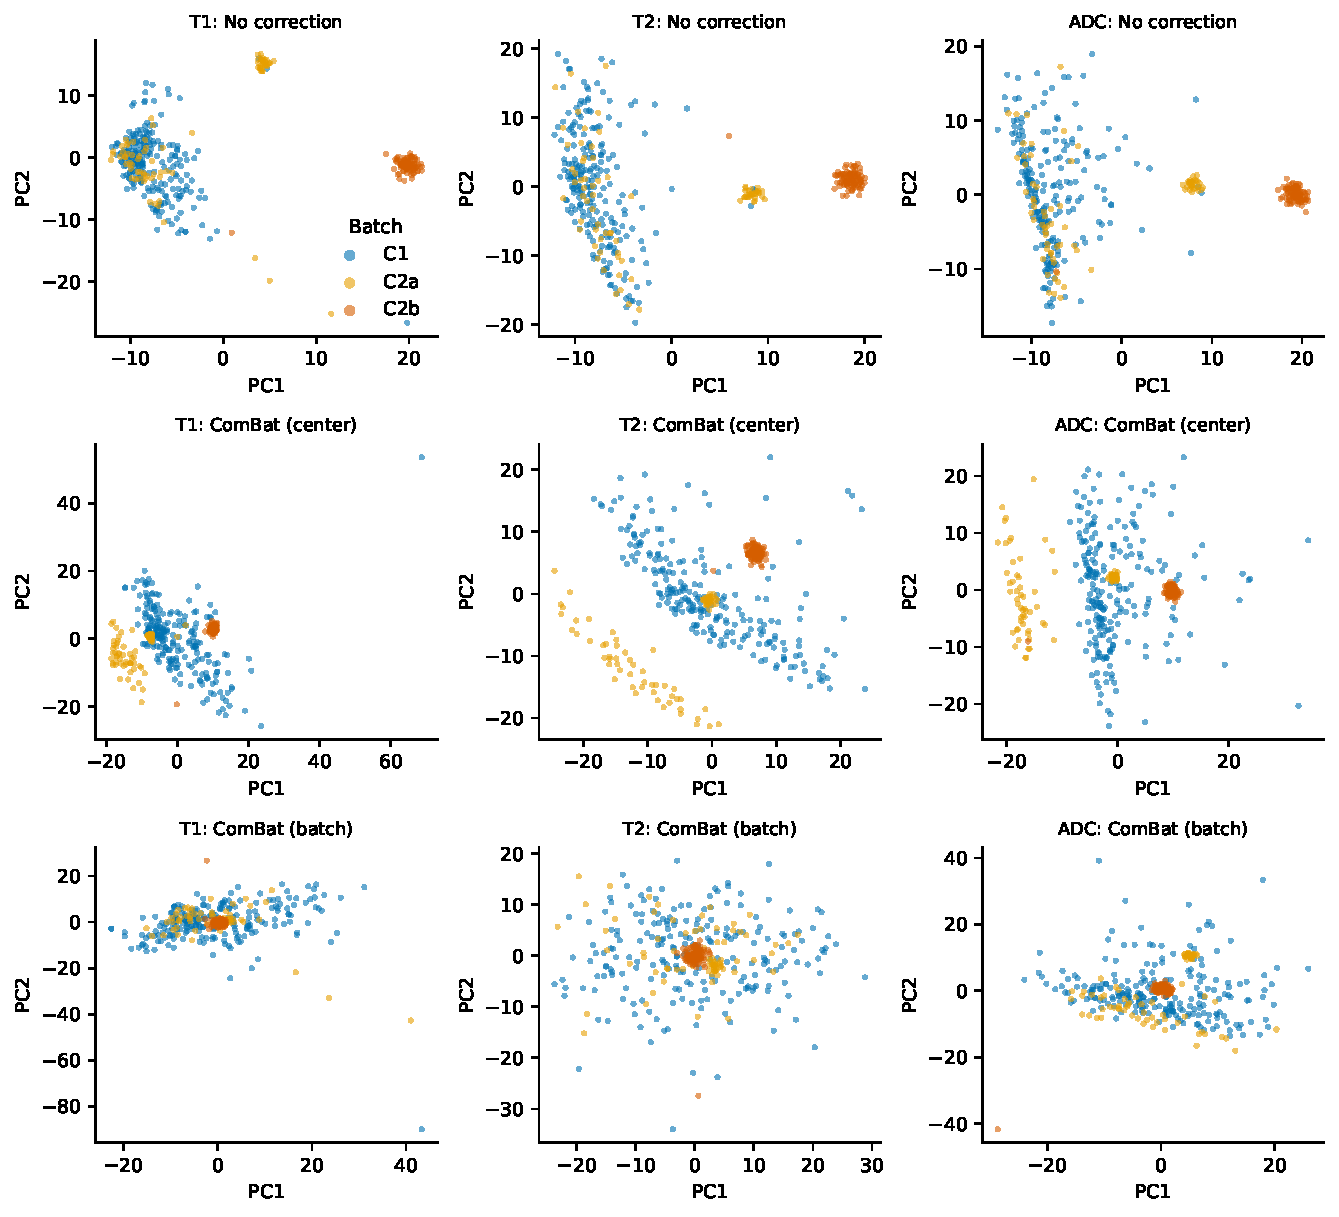
\includegraphics[width=\linewidth]{figures/harm_pca_by_batch.pdf}
\caption{First two principal components of each MRI sequence, colored by
acquisition batch, before correction (top), after ComBat by hospital center
(middle) and after ComBat by acquisition batch (bottom).}
\label{fig:ue-harm-pca}
\end{figure}

\begin{figure}[htbp]
\centering
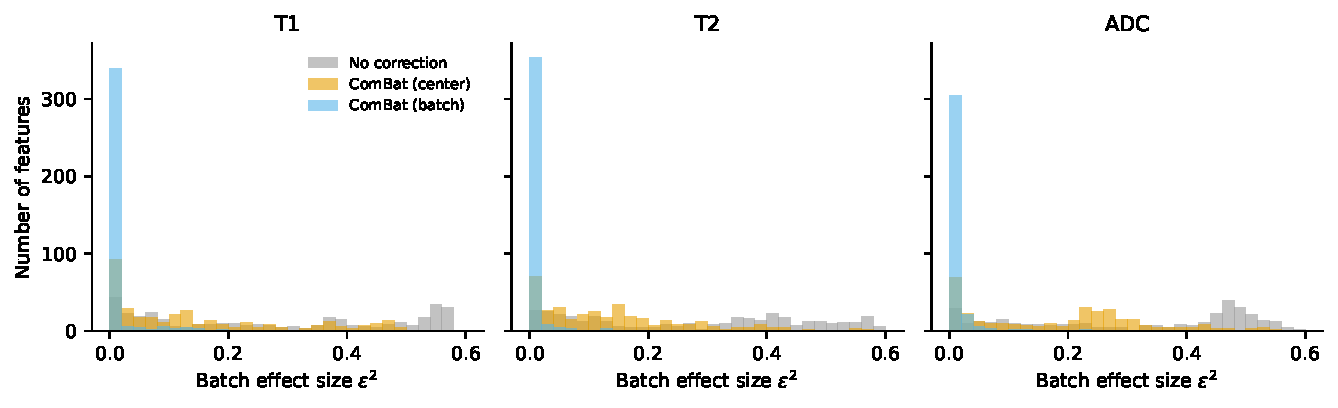
\includegraphics[width=\linewidth]{figures/harm_effectsize_hist.pdf}\\[2pt]
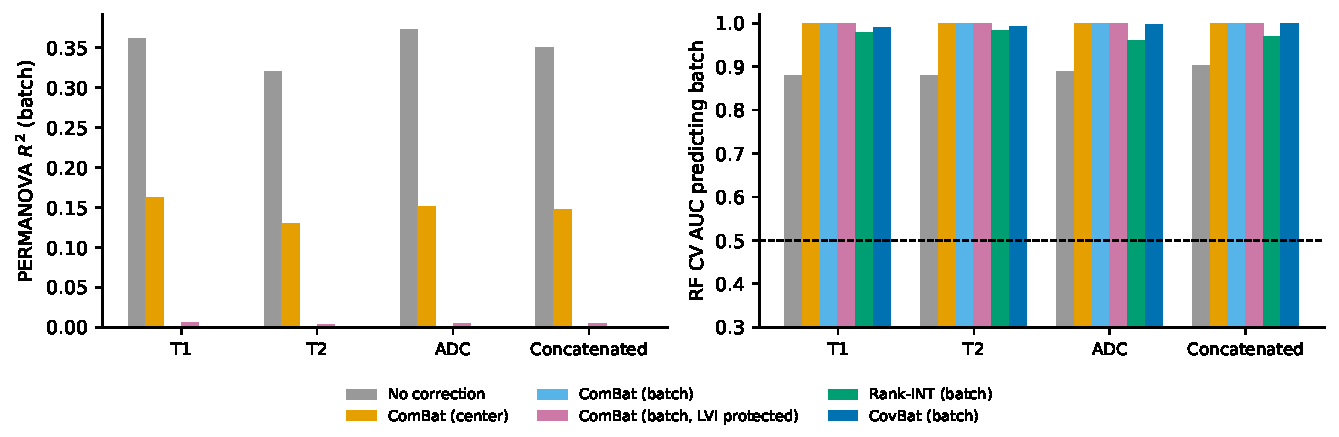
\includegraphics[width=\linewidth]{figures/harm_multivariate.pdf}
\caption{Harmonization tests. Top: distribution of feature-wise batch effect
sizes ($\epsilon^2$). Bottom: PERMANOVA $R^2$ of batch and cross-validated
random-forest AUC for predicting batch, for each strategy.}
\label{fig:ue-harm-mv}
\end{figure}

\paragraph{MOFA representation.}
On the primary harmonized data, MOFA retained eight factors that explained
46\%, 48\% and 45\% of the variance of T1, T2 and ADC
(Figure~\ref{fig:ue-mofa}). Factor~1 was shared by all three sequences.
Factors 2--3 were T1-specific, factors 4 and 8 mainly T2, and factors 5--7
mainly ADC (with a T2 contribution to 6--7). Without correction, or with
ComBat by center, one factor was almost entirely a batch factor
($\epsilon^2=0.58$ and $0.61$). After ComBat by batch, the largest factor
location effect was $\epsilon^2=0.07$ (Figure~\ref{fig:ue-mofa-batch}).
However, C2b patients had up to 12-fold smaller spread on the shared factors
than C1 patients. Excluding C2b reduced this ratio to 2.4, and the
random forest still predicted batch from the factors (AUC 0.99).

\begin{figure}[htbp]
\centering
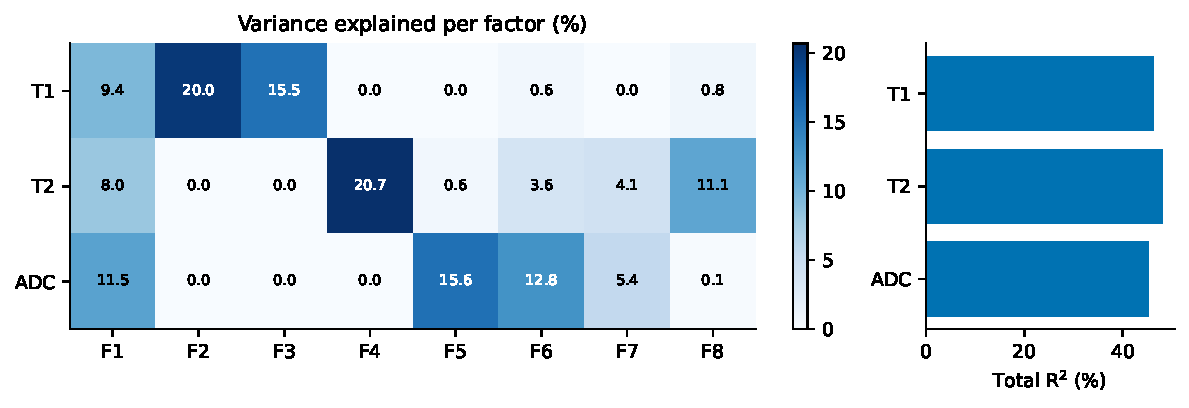
\includegraphics[width=0.85\linewidth]{figures/mofa_variance_explained.pdf}
\caption{Variance explained (\%) by each MOFA factor in each MRI sequence
(primary harmonization).}
\label{fig:ue-mofa}
\end{figure}

\begin{figure}[htbp]
\centering
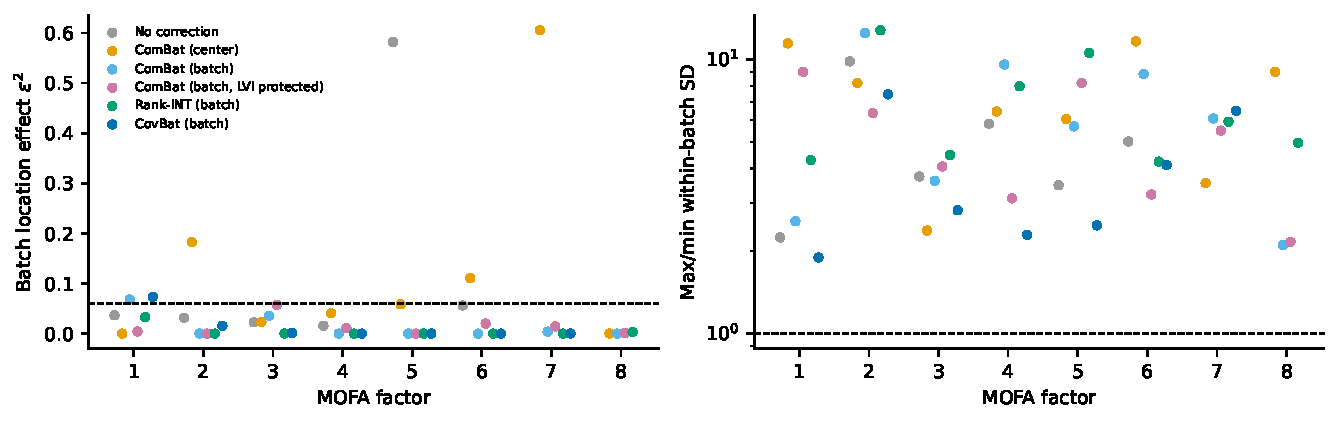
\includegraphics[width=\linewidth]{figures/mofa_factor_batch_assoc.pdf}
\caption{Batch association of the MOFA factors under each harmonization
strategy: location ($\epsilon^2$, left) and the ratio of largest to smallest
within-batch SD (right).}
\label{fig:ue-mofa-batch}
\end{figure}

\paragraph{Cluster selection and stability.}
Table~\ref{tab:ue-k} and Figure~\ref{fig:ue-k} summarize the internal
validation. Silhouette widths were low for every $k$ (0.22--0.24),
indicating weak separation. The partitions with $k\ge4$ isolated a cluster
of fewer than 10\% of patients (for $k=4$, 37 patients, 35 of them LVI-positive). This
cluster is the contiguous center-2 LVI-positive block plus a few center-1
patients, so its strong LVI association (Cram\'er's $V\approx0.57$)
reflects the extraction-block structure rather than an imaging phenotype.
The composite criterion selected $k=3$, with mean subsample ARI
$0.74\pm0.23$, pairwise ARI 0.59, PAC 0.50, and cluster sizes
260/79/64. Consensus matrices (Figure~\ref{fig:ue-cons}) show a clear
two-way split between cluster~1 and clusters 2--3, with less stable
membership between clusters 2 and 3. Cluster~1 contains 98 of the 99 C2b
patients (Cram\'er's $V$ with batch 0.30; Table~\ref{tab:ue-clbatch}), the
signature of the residual covariance batch effect. The partition was only
moderately robust (Table~\ref{tab:ue-robust}). It agreed with Ward
clustering (ARI 0.59) but not with a full-covariance Gaussian mixture
(ARI 0.02), and its agreement with partitions from alternative
harmonizations was low (ARI 0.17--0.42). In center~1 alone, the criterion
selected $k=2$ (silhouette 0.18, ARI 0.76, PAC 0.38). These two clusters
were not associated with LVI ($V=0.02$, $p=0.75$).

\begin{table*}[t]
\centering
\scriptsize
\caption{Internal validation of $k$-means partitions of the MOFA factor scores (primary harmonization).}
\label{tab:ue-k}
\resizebox{\linewidth}{!}{%
\begin{tabular}{rrrrrrlrrr}
\toprule
$k$ & Silh. & ARI (vs full) & ARI (pairwise) & PAC & Min.\ prop. & Sizes & $V_{\text{batch}}$ & $V_{\text{LVI}}$ & Score \\
\midrule
2 & 0.223 & 0.52 $\pm$ 0.48 & 0.39 & 0.58 & 0.23 & 312/\allowbreak 91 & 0.30 & 0.07 & 0.19 \\
\textbf{3} & 0.226 & 0.74 $\pm$ 0.23 & 0.59 & 0.50 & 0.16 & 64/\allowbreak 79/\allowbreak 260 & 0.30 & 0.09 & 0.67 \\
4 & 0.224 & 0.67 $\pm$ 0.19 & 0.58 & 0.53 & 0.09 & 37/\allowbreak 230/\allowbreak 78/\allowbreak 58 & 0.47 & 0.57 & -- \\
5 & 0.235 & 0.73 $\pm$ 0.21 & 0.60 & 0.46 & 0.01 & 3/\allowbreak 225/\allowbreak 80/\allowbreak 58/\allowbreak 37 & 0.48 & 0.57 & -- \\
6 & 0.229 & 0.70 $\pm$ 0.14 & 0.61 & 0.40 & 0.01 & 206/\allowbreak 46/\allowbreak 3/\allowbreak 70/\allowbreak 33/\allowbreak 45 & 0.53 & 0.58 & -- \\
7 & 0.239 & 0.67 $\pm$ 0.16 & 0.61 & 0.37 & 0.01 & 39/\allowbreak 36/\allowbreak 34/\allowbreak 33/\allowbreak 61/\allowbreak 196/\allowbreak 4 & 0.55 & 0.58 & -- \\
8 & 0.219 & 0.62 $\pm$ 0.11 & 0.59 & 0.32 & 0.01 & 34/\allowbreak 62/\allowbreak 40/\allowbreak 135/\allowbreak 66/\allowbreak 3/\allowbreak 35/\allowbreak 28 & 0.66 & 0.60 & -- \\
\bottomrule
\end{tabular}}
\par\smallskip\parbox{0.95\linewidth}{\footnotesize ARI: mean $\pm$ SD over 200 subsamples of 80\%; PAC: proportion of consensus indices in (0.1, 0.9); Score: composite rank criterion (partitions with a cluster $<$10\% excluded). Bold: selected $k$.}
\end{table*}


\begin{figure}[htbp]
\centering
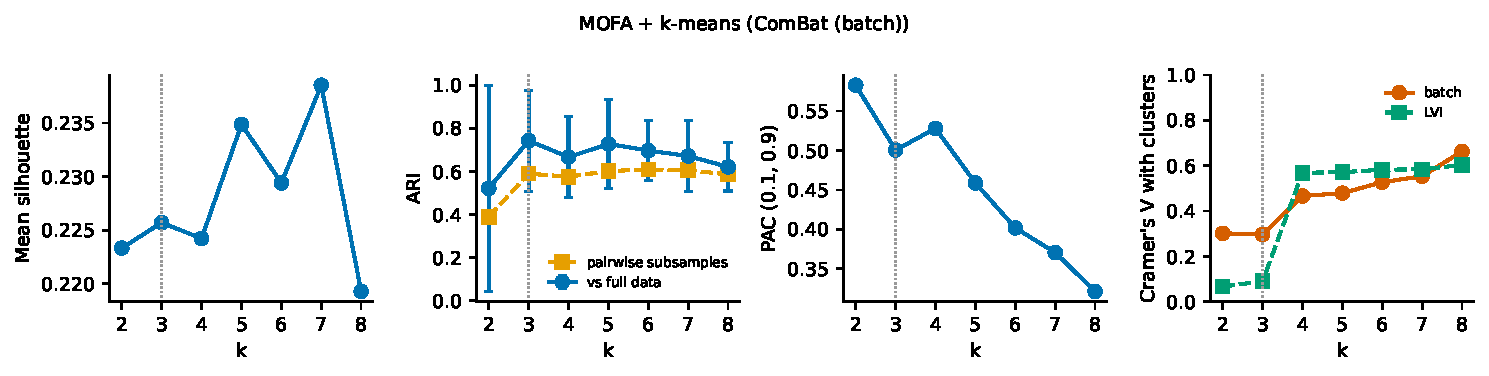
\includegraphics[width=\linewidth]{figures/cluster_selection.pdf}
\caption{Selection of $k$ on the primary MOFA representation: mean
silhouette; ARI of subsample partitions with the full-data partition
(mean $\pm$ SD) and between subsamples; PAC; and Cram\'er's $V$ of the
partition with acquisition batch and LVI. The dotted line marks the selected
$k=3$.}
\label{fig:ue-k}
\end{figure}

\begin{figure}[htbp]
\centering
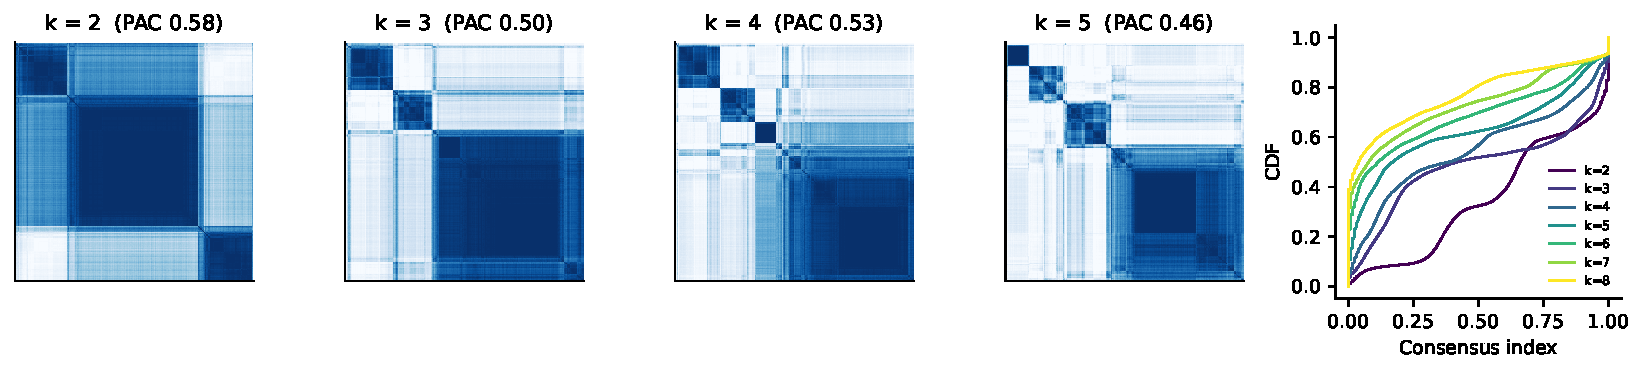
\includegraphics[width=\linewidth]{figures/consensus_matrices.pdf}
\caption{Consensus matrices ($B=200$ subsamples of 80\%) for $k=2$--5,
ordered by average-linkage clustering of $1-M$, and the empirical CDF of the
consensus index for $k=2$--8.}
\label{fig:ue-cons}
\end{figure}

\begin{figure}[htbp]
\centering
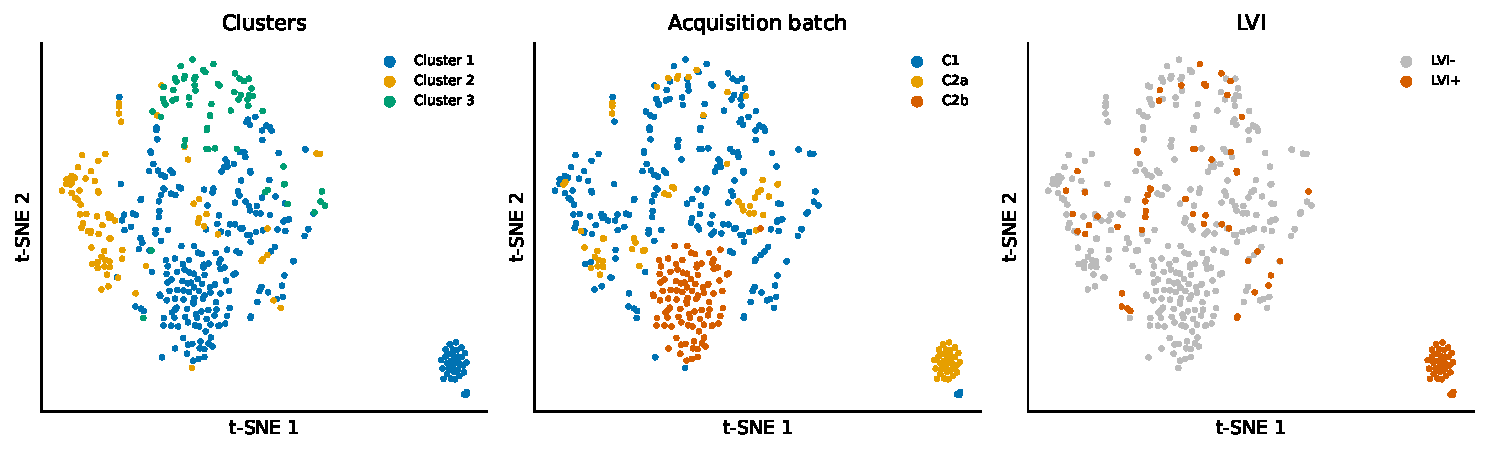
\includegraphics[width=\linewidth]{figures/cluster_tsne.pdf}
\caption{t-SNE of the MOFA factor scores (visualization only), colored by
cluster, acquisition batch and LVI.}
\label{fig:ue-tsne}
\end{figure}

\begin{table}[htbp]
\centering
\small
\caption{Primary clusters ($k=3$) by acquisition batch.}
\label{tab:ue-clbatch}
\begin{tabular}{lrrrrr}
\toprule
Cluster & C1 & C2a & C2b & Total & LVI+ (\%) \\
\midrule
1 & 112 & 50 & 98 & 260 & 24 \\
2 & 60 & 18 & 1 & 79 & 15 \\
3 & 50 & 14 & 0 & 64 & 19 \\
All & 222 & 82 & 99 & 403 & 22 \\
\bottomrule
\end{tabular}
\end{table}

\begin{table}[htbp]
\centering
\small
\caption{Robustness of the primary partition ($k=3$) to the clustering algorithm and the harmonization choice.}
\label{tab:ue-robust}
\resizebox{\linewidth}{!}{%
\begin{tabular}{lrrr}
\toprule
Comparison & $n$ & ARI & Selected $k$ (other) \\
\midrule
k-means vs Agglomerative (Ward) & 403 & 0.59 & -- \\
k-means vs Gaussian mixture & 403 & 0.02 & -- \\
ComBat (batch) vs No correction & 403 & 0.18 & 3 \\
ComBat (batch) vs ComBat (center) & 403 & 0.17 & 2 \\
ComBat (batch) vs ComBat (batch, LVI protected) & 403 & 0.32 & 2 \\
ComBat (batch) vs Rank-INT (batch) & 403 & 0.25 & 3 \\
ComBat (batch) vs CovBat (batch) & 403 & 0.42 & 2 \\
ComBat (batch) vs ComBat (batch), excl. C2b & 304 & 0.19 & 7 \\
ComBat (batch) vs Center 1 only & 222 & 0.23 & 2 \\
\bottomrule
\end{tabular}}
\end{table}


\paragraph{Radiomic characterization.}
The clusters were separated mainly by factor~4 ($\epsilon^2=0.38$; T2
grey-level non-uniformity), factor~5 ($\epsilon^2=0.28$; ADC high-grey-level
run emphasis) and factor~6 ($\epsilon^2=0.24$; ADC low-grey-level run
emphasis and low T2 intensity percentiles). Cluster~2 scored high and
cluster~3 low on factors 4 and 5, and cluster~3 was lowest on factor~6.
Cluster~1 lay near the origin on most factors, consistent with the
compressed C2b patients it contains.

\paragraph{Post-hoc analysis.}
No post-hoc variable met the retention rule (Table~\ref{tab:ue-posthoc},
Figure~\ref{fig:ue-posthoc}). The only candidate with a non-negligible effect
was the radiologist-measured ADC value. It was lower in cluster~1 (median
0.75 vs 0.83 and 0.82 $\times10^{-3}\,$mm$^2$/s; $\epsilon^2=0.045$,
$q=0.001$), and the difference persisted after batch adjustment (nominal
$p=0.015$, $q=0.15$) and within center~1 ($p=0.003$). LVI was associated
with cluster only after batch adjustment ($q=0.003$). This association came
entirely from C2a, where all 30 LVI-positive patients fell in cluster~1. It
was absent within center~1 ($p=0.38$), so we regard it as an artifact of the
center-2 extraction blocks. Ki-67 and ER had nominal batch-adjusted
$p<0.05$, but negligible effects ($\epsilon^2<0.01$). In explaining cluster
membership, all 21 variables together barely exceeded chance
(cross-validated macro-AUC 0.55). ADC alone reached 0.62, and batch alone
reached 0.68 (Table~\ref{tab:ue-models}). For the center-1 clusters, DWI
hyperintensity (98\% vs 90\%), late-arterial enhancement ratio and Ki-67
were nominally associated ($p<0.02$, $q\approx0.10$), with a joint
cross-validated AUC of 0.66.

\begin{table}[htbp]
\centering
\scriptsize
\caption{Post-hoc comparison of clinical, imaging-report and pathology variables across the primary clusters.}
\label{tab:ue-posthoc}
\resizebox{\linewidth}{!}{%
\begin{tabular}{llrrrrr}
\toprule
Variable & Cluster 1 | 2 | 3 & Effect & $q$ & $p_{\text{adj}}$ & $q_{\text{adj}}$ & $p_{\text{C1}}$ \\
\midrule
LVI & 24\% $|$ 15\% $|$ 19\% & 0.090 ($V$) & 0.730 & $<$0.001 & 0.003 & 0.381 \\
ADC value (radiologist) & 0.75 [0.67-0.85] $|$ 0.83 [0.73-0.90] $|$ 0.82 [0.73-0.90] & 0.045 ($\epsilon^2$) & 0.001 & 0.015 & 0.154 & 0.003 \\
Maximum diameter (cm) & 3.35 [2.40-4.80] $|$ 3.70 [2.13-4.75] $|$ 2.95 [2.15-4.35] & 0.000 ($\epsilon^2$) & 0.829 & 0.655 & 0.794 & 0.585 \\
Deep myometrial invasion & 46\% $|$ 48\% $|$ 41\% & 0.046 ($V$) & 0.879 & 0.587 & 0.771 & 0.627 \\
Age (years) & 59.50 [52.00-67.00] $|$ 57.00 [52.00-67.50] $|$ 58.50 [52.00-66.00] & 0.000 ($\epsilon^2$) & 0.904 & 0.744 & 0.822 & 0.941 \\
Postmenopausal & 54\% $|$ 47\% $|$ 58\% & 0.069 ($V$) & 0.781 & 0.236 & 0.550 & 0.064 \\
Tumour margin & 78\% $|$ 82\% $|$ 84\% & 0.063 ($V$) & 0.781 & 0.906 & 0.919 & 0.981 \\
DWI hyperintensity & 94\% $|$ 91\% $|$ 94\% & 0.043 ($V$) & 0.879 & 0.176 & 0.529 & 0.226 \\
Ascites & 29\% $|$ 28\% $|$ 20\% & 0.069 ($V$) & 0.781 & 0.478 & 0.765 & 0.582 \\
Lymph-node positive & 18\% $|$ 11\% $|$ 9\% & 0.102 ($V$) & 0.730 & 0.338 & 0.680 & 0.355 \\
Cystic/solid composition & 23/43/33 $|$ 23/49/28 $|$ 25/47/28 & 0.044 ($V$) & 0.904 & 0.529 & 0.765 & 0.113 \\
Enhancement ratio, early arterial & 0.73 [0.61-0.88] $|$ 0.73 [0.63-0.97] $|$ 0.71 [0.59-0.88] & 0.000 ($\epsilon^2$) & 0.781 & 0.356 & 0.680 & 0.640 \\
Enhancement ratio, late arterial & 0.77 [0.65-0.94] $|$ 0.83 [0.67-0.94] $|$ 0.77 [0.64-0.92] & 0.002 ($\epsilon^2$) & 0.730 & 0.136 & 0.525 & 0.090 \\
Enhancement ratio, parenchymal & 0.84 [0.71-1.09] $|$ 0.82 [0.70-1.02] $|$ 0.98 [0.72-1.18] & 0.004 ($\epsilon^2$) & 0.730 & 0.150 & 0.525 & 0.516 \\
Enhancement ratio, delayed & 0.90 [0.71-1.09] $|$ 0.93 [0.72-1.11] $|$ 0.88 [0.67-1.09] & 0.000 ($\epsilon^2$) & 0.879 & 0.680 & 0.794 & 0.910 \\
Relative T2 signal & 1.47 [1.15-1.76] $|$ 1.43 [1.17-1.68] $|$ 1.56 [1.20-1.80] & 0.000 ($\epsilon^2$) & 0.781 & 0.230 & 0.550 & 0.269 \\
T2WI signal grade & 50\% $|$ 51\% $|$ 48\% & 0.013 ($V$) & 0.975 & 0.919 & 0.919 & 0.909 \\
p53 abnormal & 49\% $|$ 48\% $|$ 50\% & 0.011 ($V$) & 0.975 & 0.547 & 0.765 & 0.924 \\
Ki-67 (\%) & 45.00 [35.00-55.00] $|$ 35.00 [30.00-50.00] $|$ 40.00 [38.75-55.00] & 0.008 ($\epsilon^2$) & 0.724 & 0.036 & 0.196 & 0.008 \\
ER (\%) & 45.00 [35.00-55.00] $|$ 45.00 [37.50-60.00] $|$ 50.00 [40.00-60.00] & 0.003 ($\epsilon^2$) & 0.730 & 0.037 & 0.196 & 0.322 \\
PR (\%) & 52.50 [40.00-65.00] $|$ 50.00 [40.00-65.00] $|$ 55.00 [40.00-70.00] & 0.000 ($\epsilon^2$) & 0.879 & 0.447 & 0.765 & 0.339 \\
\bottomrule
\end{tabular}}
\par\smallskip\parbox{0.95\linewidth}{\footnotesize Continuous: median [IQR], Kruskal--Wallis; binary: \% positive; composition: \% per category; $\chi^2$ or Monte-Carlo $\chi^2$. adj: batch-adjusted likelihood-ratio test; C1: within center 1. $q$: BH-FDR across variables. No variable met the retention rule ($q<0.05$ unadjusted and adjusted with at least a small effect).}
\end{table}

\begin{table}[htbp]
\centering
\scriptsize
\caption{Explanatory value of post-hoc variables for cluster membership (multinomial logistic regression, 10$\times$5-fold CV macro-AUC).}
\label{tab:ue-models}
\resizebox{\linewidth}{!}{%
\begin{tabular}{llrr}
\toprule
Clustering & Predictors & \# & CV AUC \\
\midrule
Primary ($k=3$) & Batch only & 3 & 0.68 $\pm$ 0.03 \\
 & Candidate variables: ADC value (radiologist) & 1 & 0.62 $\pm$ 0.04 \\
 & All post-hoc variables & 21 & 0.55 $\pm$ 0.05 \\
 & Candidate variables + batch & 4 & 0.71 $\pm$ 0.03 \\
Center 1 only ($k=2$) & Candidate variables: DWI hyperintensity, Enhancement ratio, late arterial, Ki-67 (\%) & 3 & 0.66 $\pm$ 0.06 \\
 & All post-hoc variables & 21 & 0.55 $\pm$ 0.07 \\
 & Candidate variables + batch & 4 & 0.66 $\pm$ 0.06 \\
\bottomrule
\end{tabular}}
\end{table}


\begin{figure}[htbp]
\centering
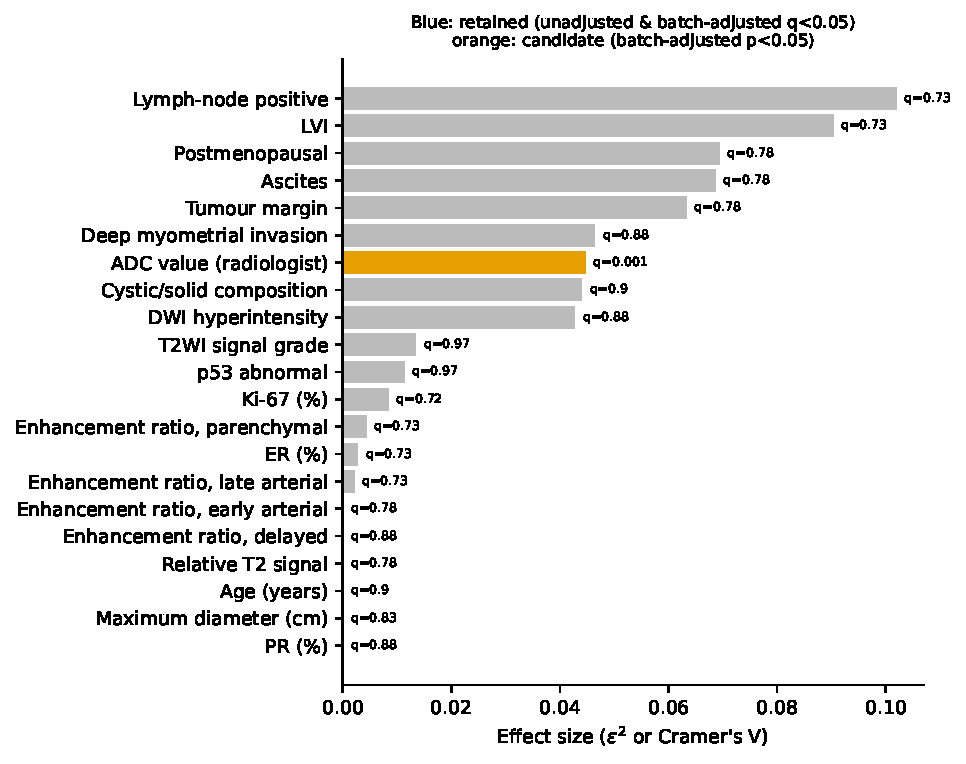
\includegraphics[width=0.55\linewidth]{figures/posthoc_effects_primary.pdf}
\hfill
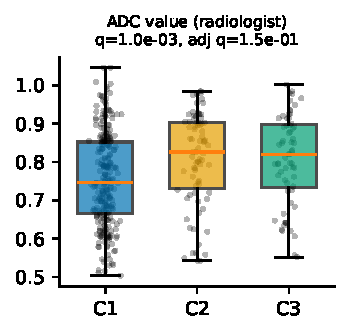
\includegraphics[width=0.3\linewidth]{figures/posthoc_retained_primary.pdf}
\caption{Post-hoc effect sizes for the primary clusters (left; orange =
candidate with nominal batch-adjusted $p<0.05$) and radiologist ADC value by
cluster (right).}
\label{fig:ue-posthoc}
\end{figure}

% ----------------------------------------------------------------------
\subsection{Discussion}
\label{sec:ue-discussion}

Harmonization was decisive in this cohort, but the relevant batch was not
the hospital. Center~2 combines at least two extraction or acquisition runs,
and ComBat by center left them intact. Defining batches from the data, and
then applying ComBat to them, removed the location and scale batch effects
that dominate the uncorrected principal components and MOFA factors. Three
findings nevertheless limit what the unsupervised clusters can show. First,
batch effects in the covariance structure remain. They are detectable by a
nonlinear classifier and visible as compressed factor scores in C2b, and
neither CovBat nor a rank-based transform removed them. Second, batch is
confounded with LVI: C2b is entirely LVI-negative, and the center-2
LVI-positive patients form their own block. No harmonization can separate
batch from outcome under this design, and protecting LVI inflates its
apparent signal \citep{nygaard2016methods}. Third, the cross-file
consistency checks suggest that patient linkage between sequences and the
clinical table may be incorrect for part of the cohort.

Within these limits, the latent space shows weak cluster structure. The
silhouette is about 0.23, and the subsamples gave a moderately stable
three-cluster partition, driven by T2 and ADC texture factors, that depends
on the harmonization choice. The clusters are not explained by the clinical,
imaging-report or pathology variables. The only consistent association is a
lower radiologist ADC value in cluster~1, which also holds within center~1.
Lower ADC is generally associated with higher cellularity, but the effect is
small. The single-center analysis, which is free of harmonization, likewise
found no LVI-related phenotype. We therefore present the clusters as
exploratory imaging phenotypes rather than clinically validated subtypes.
Before further modeling, we recommend (i) verifying the case linkage and
acquisition metadata, and harmonizing on recorded scanner and protocol
rather than inferred batches; (ii) re-extracting features with a common
discretization; and (iii) re-running the pipeline
(\texttt{code/unsupervised\_extension/run\_all.sh}), with external validation
in a cohort where LVI is not confounded with acquisition.


\bibliographystyle{plainnat}
\bibliography{reference}

\end{document}
